\subsection{Description du projet}
La societe Infineon Technologie GA propone un gateway securis\'e \cite{gateway} el cual corre con un microcontrolador \textit{AURIX TC37xEXT} para poder aumentar la conectividad de diferentes redes como el FlexRay, LIN, CAN y Ethernet dentro del automobil. El sistema operativo usado dentro de este gateway es fourni por Vector Informatik y se llama MICROSAR Classic \cite{vector.microsar}. Este sistema operativo es totalmente compatible con AUTOSAR lo cual nos deja con una ECU 100\% funcional sobre la cual se pueden correr software components (swc) compatibles con AUTOSAR. Ademas tambien se utilisa un switch ethernet securis\'e Marvell 88Q5050 que permite velocidad y ancho de banda estables con toda la seguridad que un automobil requiere.

Este software viene por defecto con un demo que permite testear la cual propone 2 use case mostrados en las figuras \ref{fig:gw-demo-uc1} y \ref{fig:gw-demo-uc2}.

\begin{figure}[!htb]
 \centering
 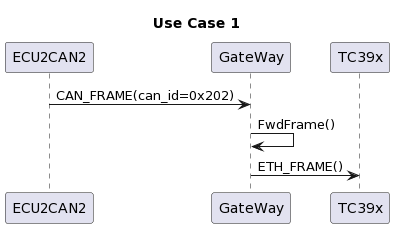
\includegraphics[width=0.5\textwidth]{img/GWUseCase1.png}
 \caption{Gateway Demo Use Case 1}
 \label{fig:gw-demo-uc1}
\end{figure}

\begin{figure}[!htb]
 \centering
 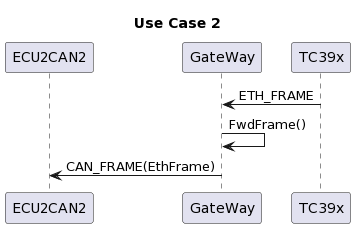
\includegraphics[width=0.5\textwidth]{img/GWUseCase2.png}
 \caption{Gateway Demo Use Case 2}
 \label{fig:gw-demo-uc2}
\end{figure}

\subsection{Objectifs du projet}

Los objetivos del proyecto son basicamente los siguientes:
- Hacer correr el Demos

Gateway Autosar
Un Gateway es tal tal y tal. Este gateway es autosar, las ventajas de que sea autosar esque puedes integrarlo  al entorno de trabajo. Por ejemplo el ethernet es buenisimo para grandes cantidades de datos como videos y procesamiento. Sin embargo nuestras ECU's pueden tener la necesidad de pedir datos a otras ecu's sin necesidad de estar conectados a la misma red.

Ahora si explico bien que es el gateway, para que sirve, como se usa en la vida real y todo eso. Ademas debo decir que el gateway viene con su propio RTOS basado en autosar y que ellos quieren hacer una demo funcional de este gatway para mostrarle a los clientes mas adelante. El gateway viene con un OS ya predefinido para ese microcon pero no arranca porque inicialmente no esta conectado a nada.